\section{Summarizing Overall Opinion}
\begin{figure}
	\centering
	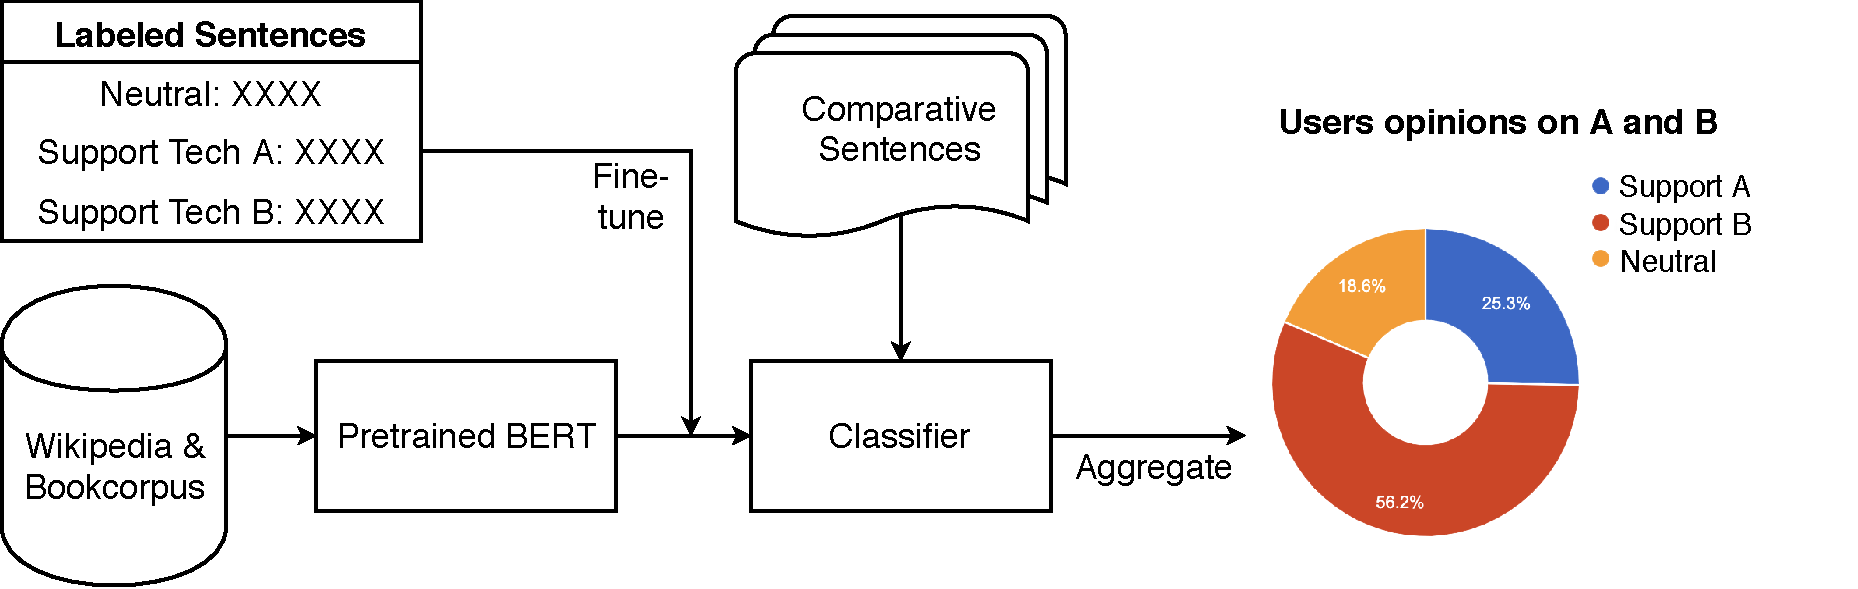
\includegraphics[width=0.45\textwidth]{figures/bert.pdf}
	\vspace{-2mm}
	\caption{\revise{Summerizing overall opinions towards each technology}}
	\label{fig:finetune}
\end{figure} 
\revise{For some comparable technologies, there may be too many comparison opinions which are too time-consuming for developers to read all of them.
Therefore, we further develop a sentiment classifier based on the BERT model~\cite{devlin2018bert} for automatically distilling the overall opinion towards the comparable technologies.
That summarization can be an important criteria for developers to determine which technology for adopting.
The general process of summarising overall opinion is shown in Fig.~\ref{fig:finetune}}

\begin{comment}
While comparing two techniques, users also would like to see an overall opinion on which technology is better or which one should they use.  
After collecting all the comparative sentences, we randomly picked several sentences and label them based on semantically which technology they think is better. After that, we use BERT\cite{devlin2018bert} model to train the labeled sentences, and manage to predict which technology the writer suggest from the comparative sentences. For each comparable technology pair, we collect all the prediction of sentences and generate an overall opinion for each pair.
\end{comment}

\begin{figure*}
	\centering
	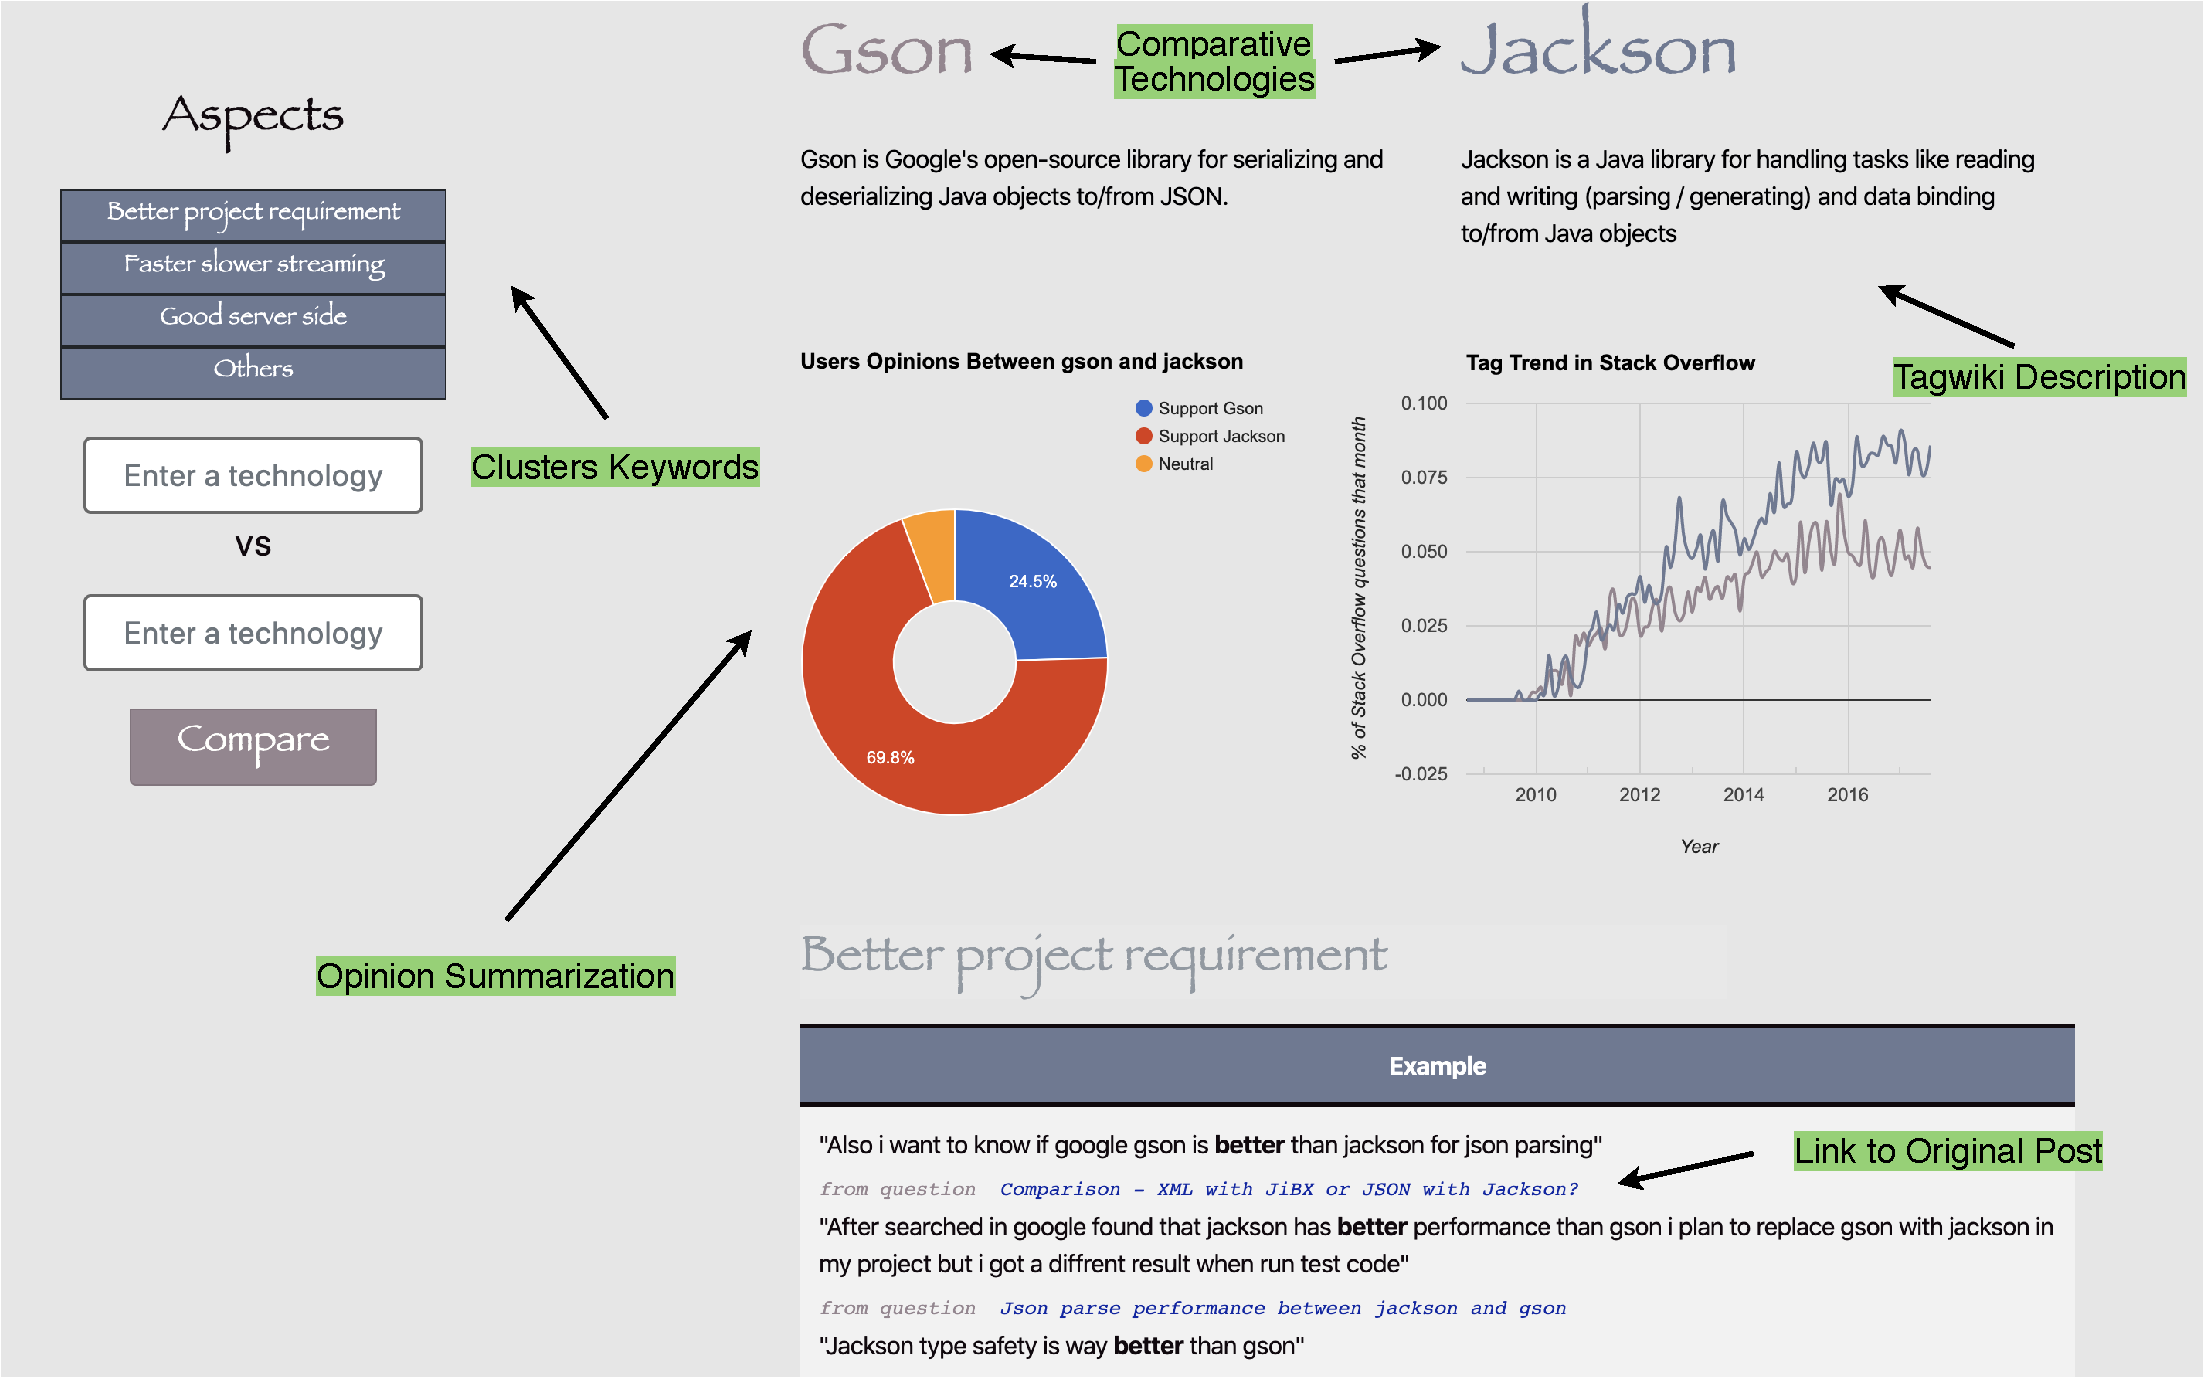
\includegraphics[height=90mm]{figures/website.pdf}
	\vspace{-3mm}
	\caption{The screenshot of our website \textit{DiffTech} and some important elements in the website \chen{1) The first sentence is a question actually that should be removed; 2) Can we find change another example that there is no explicit comparison posts? 3) For the webpage, can we add a line after the tagwiki, and a line after the trend? 4) For the trend graph, how to know which line is for which technology? 5) The clustering of this example is not good, so change another example.}}
	\vspace{-3mm}
	\label{fig:website}
\end{figure*} 

\revise{
For summarizing the overall opinions toward comparable technologies, we formulate it as a classification problem.
Given a set of comparative sentences about them, we build a classifier for identifying which technology does each sentence support.
By counting the total number of support sentences for each technology, we obtain the sentiment summarization of them.
We replace the comparable technology pairs with two unique tokens i.e., TechA (first occurrence) and TechB (second occurrence) to generalize different technology pairs.
We randomly select 801 comparative sentences and replace the comparable technology pairs with two unique tokens i.e., TechA (first occurrence) and TechB (second occurrence) to generalize different technology pairs.}

\begin{comment}
As mentioned above, we use BERT, which stands for Bidirectional Encoder Representations from
Transformers, for deploying sentence analysis. There are already plenty of pre-trained models in the market, we choose BERT because it supposed to be the first deeply bidirectional, unsupervised language representation, pre-trained using only a plain text corpus\cite{web:bertblog}. And quite a lot works have proved that BERT model \wang{find some reference} has surpassed other  transformers.
\end{comment}

\begin{comment}
\begin{figure}
	\centering
	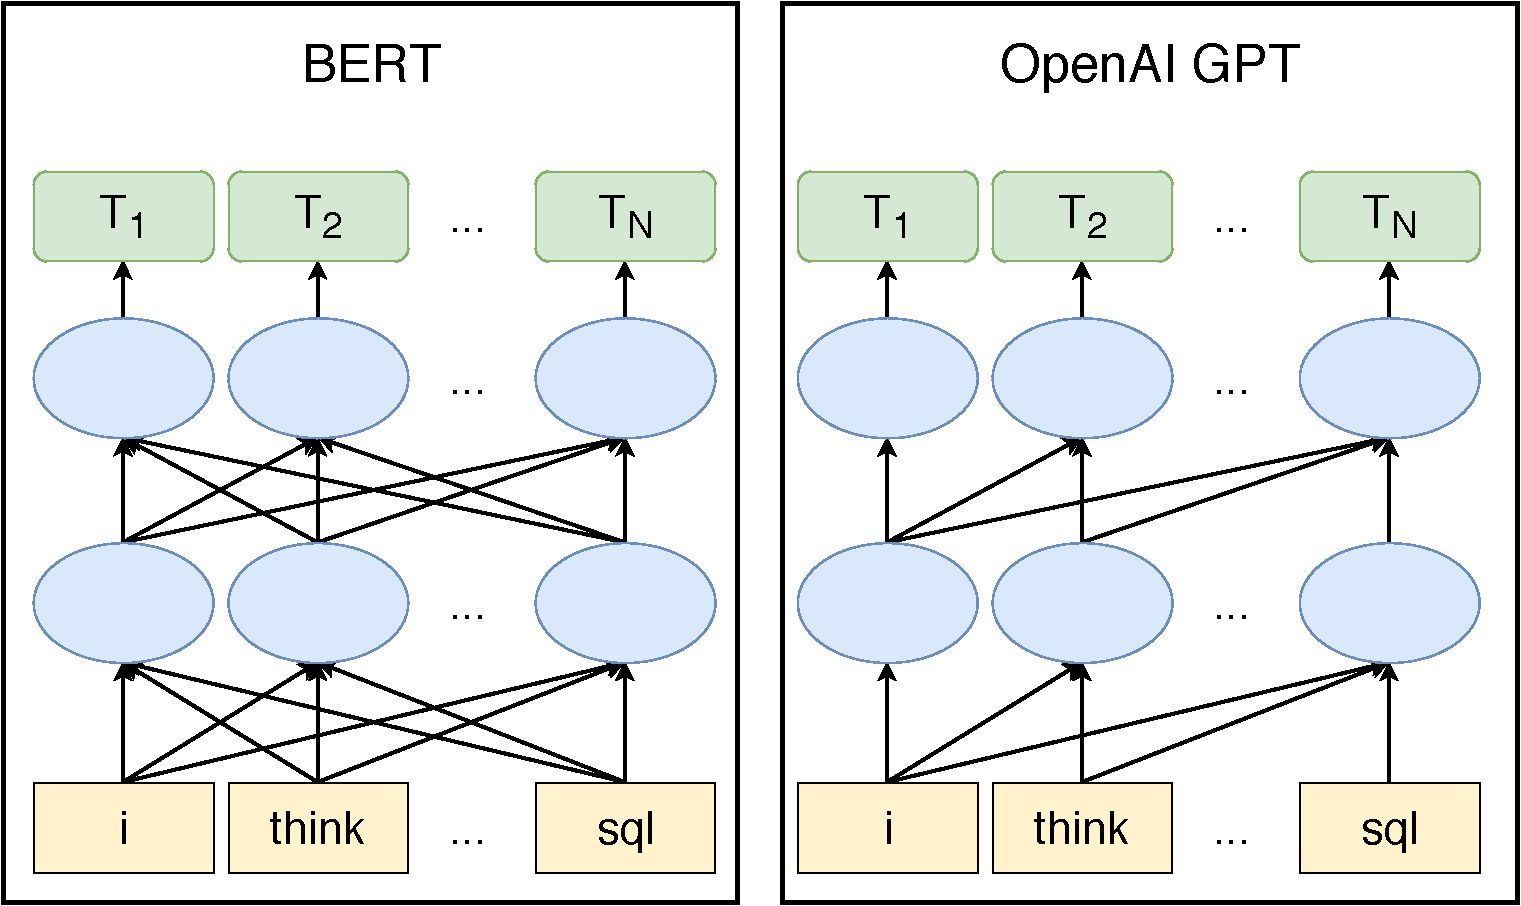
\includegraphics[height=50mm]{figures/bertmodel.pdf}
	\vspace{-3mm}
	\caption{BERT deeply bidirectional architecture compare with OpenAI GPT which is unidirectional}
	\vspace{-3mm}
	\label{fig:bertmodel}
\end{figure}
\end{comment}

%\subsection{Constructing the classifier}
%\label{sec:fineTuning}
\revise{
However, the supervised learn requires a large-scale labeled dataset which labour-extensive and time-consuming.
To overcome this issue, we adopt the state-of-the-art model, BERT for this work.
BERT (Bidirectional Encoder Representations)~\cite{devlin2018bert} is \wang{the first deeply bidirectional unsupervised language representation, pre-trained using only a plain text corpus\cite{web:bertblog}. 
For each word, BERT considers its different meanings in different contextual environments. For example, the word `chair' would have same representation in `seat a the chair' and `the chair of the committee' for a context-free models. A contextual model like BERT would have one representation of each word that is based on the other words in its surroundings.  BERT also introduce the ``masked language modeling'', which is to make sure BERT is a deep bidirectional representation. While doing the training, the model will randomly mask some percentage of the input tokens, and predict them. For example, the \textbf{Input} is ``A Lady went to the [MASK1]. She bought a [MASK2] of pork belly.'' and the \textbf{Labels} are ``MASK1=butcher,MASK2=tray''. Those features make BERT different but powerful than other pre-trained representations. }
In addition, Google release a pretrained BERT model~\cite{web:bertmodel} based on the large-scale corpus including Wikipedia and BookCorpus~\cite{moviebook} which contains 2,500 million words from English wikipedia sentences and 800 million words from 11,038 unpublished books.
As the pretrained model is well trained based on such big data and long time, it already encodes a lot of information about our general language. 
To leverage that learned knowledge, we only fine tune the pretrained BERT model by adding a new layer on the top of it.
We freeze the parameters of existing pretrained model but only train the final layer based on a small manually-labeled dataset for adapting it with domain-specific information.
}

\begin{comment}
BERT has already been trained with large amount of plain text, so we only need to provide a small set of data to BERT for fine-tune. And expect it the model to return its predictions. 
From all the comparative sentences, we randomly select around 800 sentences as training corpus. We firstly replace the comparable technology pairs with two unique tokens e.g. Tech A and Tech B, to reduce the ambiguity of different technology pairs.  For each sentence, we have three possible labels as 0, 1, 2. A sentence will be labeled as 0 if itself is neutral and we can't see which technology is better. Label 1 means that we can predict that tech A is better than tech B on some certain aspect or overall speaking, whereas label 2 means the opposite. Table~\ref{tab:label} shows some sample sentences we labeled and all the labeled sentences construct the training corpus for fine-tuning.
\end{comment}



\begin{comment}
Then, we further process the sentences to structures that BERT can understand. The process start with breaking sentences into tokens and add start mark "CLS" and end mark "SEP"to all tokenized sentences. We also add the index and segment id from words in sentences to the input data based on the provided BERT vocabulary file.

We use the TensorFlow estimator to train and predict data. After preprocing the data input, we load the BERT model and create a new layer on the top of it. The new layer then get trained, and after a few epoch of training, the new model will be able to predict sentences based on the training samples.

\end{comment}



